\documentclass{article}

\usepackage[dvips]{graphicx}

\usepackage{amsmath}
\usepackage{natbib}
\usepackage{url}

\usepackage{algorithmic}

\newenvironment{eqnnon}{\begin{equation}}{\end{equation}}

\bibliographystyle{apa}

\title{Solving for multi-class using orthogonal coding matrices}

\author{Peter Mills}

\begin{document}

\maketitle

\begin{center}
	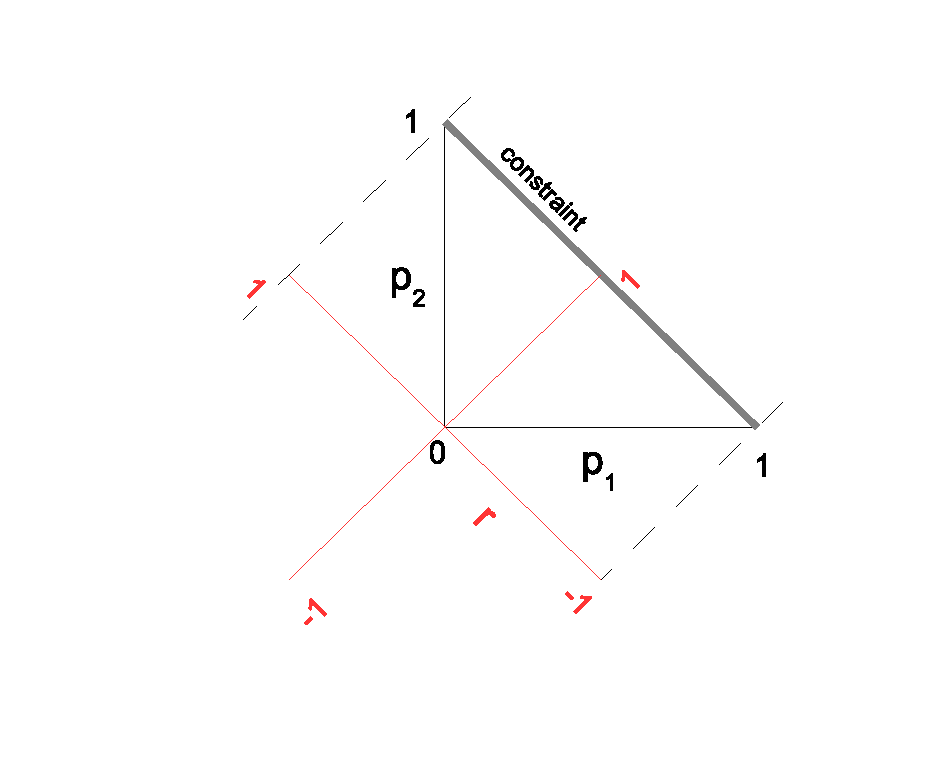
\includegraphics[width=0.6\textwidth]{../multi2/binary_class_map}
\end{center}

\section*{Abstract}

\input{orthogonal_abstract.txt}

\section*{Keywords}
\textbf{multi-class classification, 
	conditional probabilities,
	SVM,
	error-correcting codes,
	constrained linear least squares}

\tableofcontents

\section*{List of symbols}
\addcontentsline{toc}{section}{List of symbols}

\begin{tabular}{lll}
symbol & description & first used \\\hline
	$c$ & class & (\ref{min_dist}) \\
	$\vec x$ & test point & (\ref{min_dist})\\
	$A = \lbrace a_{ij} \rbrace$ & coding matrix & (\ref{min_dist})\\
	$\vec r = \lbrace r_i \rbrace$ & vector of binary decision functions & (\ref{rdef}) \\
	$P_i(c | \vec x)$ & conditional probability of $i$th binary classifier & (\ref{rdef})\\
	$p_j = p(j | \vec x)$ & multi-class conditional probability & (\ref{multiclass})\\
	$m$ & number of classes & (\ref{multiclass})\\
	$n$ & number of binary classifiers & (\ref{multiclass}) \\
	$I$ & identity matrix & (\ref{orthogonal})\\
	$t$ & whole number for enumerating cases & Section \ref{construction} \\
	$p(\vec x)$ & prior distribution & (\ref{theorem}) \\
	$\lbrace \vec x_i:y_i \rbrace$ & a set of training samples & (\ref{theorem}) \\
	$N$ & number of training samples/conditional probabilities & (\ref{theorem})\\
	$\delta$ & Kronecker delta & (\ref{theorem}) \\
	$i_0$ & rank of first winning probability & (\ref{prob_val1})\\
\end{tabular}




\section{Introduction}

Many methods of statistical classication can only discriminate between two classes. 
Examples include lineear classifiers such as perceptrons and logistic regression \citep{Michie_etal1994}, 
piecewise linear classifiers \citep{Herman_Yeung1992,Mills2011},
as well as support vector machines \citep{kernel_intro}.
There are many ways of generalizing binary classification to 
multi-class.
Three of the most common are one versus one, one versus the rest and 
error-correcting coding matrices \citep{Hsu_Lin2002}.
Here we are interested in the error-correcting coding matrices
\citep{Dietterich_Bakiri1995, Windeatt_Ghaderi2002} and
rather than use a random coding matrix we are interested in one that is
more carefully designed.

In error-correcting coding, there is a coding matrix, $A$, that specifies
how the set of multiple classes is partitioned.
Typically, the class of the test point is determined by the distance between
a row in the matrix and a vector of binary {\it decision functions}:
\begin{eqnnon}
	c(\vec x) = \arg \min_i | \vec a_i - \vec r(\vec x) |
	\label{min_dist}
\end{eqnnon}
where $\vec a_i$ is the $i$th row of the coding matrix and $\vec r$
is a vector of decision functions at {\it test point}, $\vec x$.
If we take the upright brackets as a Euclidean distance, and assume that
each partition partitions all of the classes, that is, there are no zeroes
in $A$, then this reduces to a {\it voting} solution:
\begin{equation}
	c = \arg \max A \vec r \label{voting}
\end{equation}
Both \citet{Allwein_etal2000} and \citet{Windeatt_Ghaderi2002} show that to
maximize the accuracy of an error-correcting coding matrix, the distance
between each row, $|\vec a_i - \vec a_j|_{i \ne j}$ should be as
large as possible.
Using the same assumptions, this reduces to:
\begin{eqnnon}
	\min |\vec a_i \cdot \vec a_j|_{i \ne j}
\end{eqnnon}
In other words, the coding matrix, $A$, should be orthogonal.
This approach to the multi-class problem will be described in detail in this note.

\section{Algorithm}

We wish to design a set of $n$ binary classifiers, each of which return a 
decision function:
\begin{eqnnon}
r_j(\vec x) = P_j(-1 | \vec x) - P_j(+1 | \vec x)
\label{rdef}
\end{eqnnon}
where $P_j(c | \vec x)$ is the conditional probability of the $c$th class of
the $j$th classifier.
Each binary classifier partitions a set of $m$ classes such that for a
given test point, $\vec x$:
\begin{eqnnon}
	\sum_{i=1}^m a_{ij} p_i = r_j; ~~~ j=[1..n]
\label{multiclass}
\end{eqnnon}
where $A=\lbrace a_{ij} \in \lbrace -1, +1 \rbrace  \rbrace$ is a {\it coding
matrix} and $p_i = p(i | \vec x)$ is the 
conditional  probability of the $i$th class.
In vector notation:
\begin{equation}
	A^T \vec p = \vec r \label{inverse}
\end{equation}
The more general case where a class can be excluded, that is the coding 
may include zeroes, $a_{ij} \in \lbrace -1, 0, +1\rbrace$,
will not be addressed here.

Note that this assumes that the binary decision functions, $\vec r$,
estimate the conditional probabilities perfectly.
In practice
there are a set of constrainsts that must be enforced
because $\vec p$ is only allowed to take on certain values.
Thus, we wish to solve the following minimization problem:
\begin{equation}
	\arg \min_{\vec p} | A^T \vec p - \vec r | \label{minimization}
\end{equation}
\begin{eqnarray}
	\sum_{i=1}^m p_i & = & 1 \label{normalization}\\
	p_i & \ge & 0; ~~~ i=[1..m] \label{nonnegative}
\end{eqnarray}

If $A$ is orthogonal,
\begin{eqnnon}
	A A^T = n I
	\label{orthogonal}
\end{eqnnon}
where $I$ is the $m \times m$ identity matrix,
then the unconstrained minimization problem is easy to solve. 
Note that the voting solution in (\ref{voting}) is now equivalent to
the inverse solution in (\ref{inverse}).
%and also that, unless coding matrix, $A$, is 
%square, $n=m$, it is only orthogonal in one direction.
This allows us to determine the class easily, but we also wish to solve for
the probabilities, $\vec p$, so that none of the constraints in 
(\ref{normalization}) or (\ref{nonnegative}) are violated.
Probabilities are useful for gauging the accuracy of a classification result
when its true value is unknown and for recalibrating an image derived from
statistical classification \citep{Fawcett2006,Mills2009,Mills2011}.

The orthogonality property allows us to reduce the minimization problem 
in (\ref{minimization}) to something much simpler:
\begin{eqnnon}
	\arg \min_{\vec p} | \vec p - \vec p_0 |
\end{eqnnon}
where $\vec p_0 = A \vec r/n$ with the constraints in (\ref{normalization}) and
(\ref{nonnegative}) remaining the same.
Because the system has been rotated and expanded, the non-negativity 
constraints in (\ref{nonnegative}) remain orthogonal, meaning they are 
independent: enforcing one by setting one of the probabilities to zero, 
$p_k=0$ for example, shouldn't otherwise affect the solution.
This still leaves the normalization constraint in (\ref{normalization}):
the problem, now strictly geometrical, is comprised of finding the point nearest $p_0$ on the diagonal hyper-surface that bisects the unit hyper-cube.

Briefly, we can summarize the algorithm as follows:
1. move to the nearest point that satisfies the normalization constraint,
(\ref{normalization}); 2. if one or more of the probabilities is negative,
move to the nearest point that satisfies both 
the normalization constraint
and the non-negativity constraints, (\ref{nonnegative}), for the negative probabilities;
3. repeat step 2.
More formally, let $\vec 1$ be a vector of all $1$'s:
\begin{itemize}
	\item $i=0$; $m_0=m$
	\item while $\exists k \, p_{ik} < 0 \lor \vec p_i \cdot \vec 1 \ne 1$:
	\begin{itemize}
		\item if $\vec p_i \cdot \vec 1 \ne 1$ then 
		$\vec p_{i+1} = \vec p_i + (\vec p_i \cdot \vec 1 - 1)/m_i$
		\item let $K$ be the set of $k$ such that $p_{i+1,k} < 0$
		\item for each $k$ in $K$:
		\begin{itemize}
			\item $p_k=0$
			\item Remove $k$ from the problem
		\end{itemize}
		\item $m_{i+1}=m_i-|K|$
		\item $i=i+1$
	\end{itemize}
\end{itemize}

Note that resultant direction vectors for each step form an orthogonal set.
For instance, suppose $m_0=4$ and after enforcing the normalization constraint,
the first probability is less than zero, $p_{1,1} < 0$,
then the direction vectors for the two motions are:
\begin{eqnnon}
	\frac{1}{2}[1, 1, 1, 1] \cdot \frac{1}{2\sqrt{3}} [-3, 1, 1, 1] = 0
\end{eqnnon}

More generally, consider the following sequence of vectors:
\begin{eqnnon}
	v_{ij} = \frac{1}{\sqrt{(m-i)^2-2(m-i-1)}} \left \lbrace \begin{array}{rl}
			0; & j < i \\
			-m+i+1; & j=i \\
			1; & j > i
		\end{array} \right .
\end{eqnnon}
where $i \in [1, m]$ and $j \in [1, m]$. \citep{Boyd_Vandenberghe2004}


\section{Constructing the coding matrix}

\label{construction}

Finding an $A$ such that $A A^T = n I$ and $a_{ij} \in \lbrace -1, 1, \rbrace$
is quite a difficult combinatorial problem.
Work in signal processing may be of limited applicability because coding
matrices are typically comprised of $0$'s and $1$'s 
rather than $-1$'s and $+1$'s \citep{Hedayat_etal1999,Panse_etal2014}.
Moreover, there are further restrictions needed here: 
each row as well as each column must have
both positive and negative elements, or:
\begin{eqnarray}
	\left | \sum_{j=0}^n a_{ij} \right | < n; & ~~~ & i=[1..m] \label{restriction}\\\nonumber
	\left | \sum_{i=0}^m a_{ij} \right | < m; & ~~~ & j=[1..n] 
\end{eqnarray}

A simple method of designing an orthogonal $A$ is using harmonic series.
Consider the following matrix for five classes ($m=5$) 
and eight binary classifiers ($n=8$):
\begin{equation}
	A = \left [ \begin{array}{rrrrrrrr}
			-1 & -1 & -1 & -1 & 1 & 1 & 1 & 1 \\
			-1 & -1 & 1 & 1 & -1 & -1 & 1 & 1 \\
			-1 & 1 & -1 & 1 & -1 & 1 & -1 & 1 \\
			 1 &  1 & -1 & -1 & -1 & -1 & 1 & 1 \\
			-1 & 1 & 1 & -1 & -1 & 1 & 1 & -1 
	\end{array} \right ]
	\label{harmonic}
\end{equation}
This will limit the size of $m$ relative to $n$; more precisely:
$m \le \lfloor 2 \log_2 n \rfloor - 1$. Moreover, only certain values of $n$
will be admitted: $n=2^t$ where $t$ is a whole number.

The first three rows in (\ref{harmonic}) comprise a Walsh-Hadamard code \citep{Arora_Barak2009}.
A square ($n=m$) orthogonal coding matrix is called a Hadamard matrix
\citep{Sylvester1867}.
It can be shown that besides $n=1$ and $n=2$, only Hadamard matrices of size
$n=4t$ exist,  
and it is still unproven that examples exist for all values of $t$
\citep{Hedayat_Wallis1978}.
A very simple, recursive method exists to generate matrices of size $n=t^2$ 
\citep{Hedayat_Wallis1978} but without the properties in (\ref{restriction}).
Such a matrix will include a ``harmonic series'' of the same type as in
(\ref{harmonic}).

%Noting which versions of $A$ are degenerate (equivalent) can help us whittle
%away at the problem:
%\begin{itemize}
%	\item $-A$ is equivalent to $A$
%	\item re-arranging either the rows or columns of $A$ makes an equivalent $A$: $T_{ij} A$ or $A T_{ij}^T$ are both equivalent to $A$ where $T_{ij}$ is the elementary matrix which exchanges rows $i$ and $j$
%\end{itemize}

To compute the results in this note, orthogonal coding matrices were generated
using a ``greedy'' algorithm.
We choose $n$ to be the smallest multiple of $4$ equal to or larger than $m$.
and start with an empty matrix.
Candidate vectors containing both positive and negative elements 
are chosen at random to comprise a row of the matrix but never repeated.
If the candidate vector is orthogonal to existing rows, then it is added to the matrix.
The process is repeated until the matrix is filled.
A full matrix is almost always returned especially if $m<n$.
The matrix is then checked to ensure that 
each column contains both positive and negative elements.

Obviously, this method of finding orthogonal coding matrices
will only work for relatively few classes.
More work will need to be done to find efficient methods
of generating these matrices
if they are to be efficiently applied to problems with a large number of classes.


\section{Results}

\begin{table}
\caption{Speed and skill of multi-class classification results; Brier score for conditional probability estimates.}\label{class_results}
\begin{tabular}{|ll|lll|}
\hline
dataset & method & time (s) & U.C. & Brier score \\
\hline\hline
shuttle & 1 vs. 1 & $       7.6\pm     0.2$ & $     0.954\pm   0.004$ & $   0.032\pm   0.002$ \\
& ortho. & $     15.7\pm     0.3$ & $     0.944\pm   0.003$ & $   0.038\pm   0.002$\\
\hline
segment & 1 vs. 1 & $        0.240\pm   0.008$ & $    0.928\pm    0.014$ & $    0.088\pm   0.007$ \\
& ortho. & $        0.27\pm   0.01$ & $     0.923\pm    0.014$ & $   0.088\pm    0.007$\\
\hline
sat & 1 vs. 1 & $       2.50\pm    0.07$ & $     0.803\pm   0.007$ & $    0.144\pm   0.003$ \\
& ortho. & $      4.51\pm    0.08$ & $    0.797\pm   0.009$ & $    0.148\pm   0.003$\\
\hline
pendigits & 1 vs. 1 & $      1.46\pm    0.04$ & $     0.987\pm   0.003$ & $   0.031\pm   0.002$ \\
 & ortho. & $      4.3\pm      0.1$ & $     0.982\pm   0.003$ & $   0.037\pm   0.002$\\
\hline
usps & 1 vs. 1 & $        44.3\pm     0.4$ & $     0.927\pm   0.008$ & $   0.067\pm   0.003$ \\
& ortho. & $      81.0\pm     0.6$ & $      0.921\pm   0.008$ & $   0.071\pm   0.003$\\
\hline
vehicle & 1 vs. 1 & $      0.068\pm   0.004$ & $    0.634\pm    0.024$ & $    0.272\pm   0.006$ \\
& ortho. & $      0.075\pm   0.005$ & $    0.627\pm     0.030$ & $    0.276\pm   0.009$\\
\hline
\end{tabular}


\end{table}

Orthogonal error correcting codes were tested on six different datasets:
two for digit recognition--``pendigits'' \citep{Alimoglu1996} and
``usps'' \citep{Hull1994}, the space shuttle control dataset--``shuttle''
\citep{King_etal1995}, a satellite land recognition
dataset--``sat'', a similar dataset for image recognition--``segment'',
and a dataset for vehicle recognition--``vehicle'' \citep{Siebert1987}.
The last four are borrowed from the ``statlog'' project \citep{King_etal1995,Michie_etal1994}.

The method was compared with a technique that solves the ``one versus one'' 
partitioning using matrix inversion \citep{Wu_etal2004}.
Both techniques were applied to support vector machines (SVMs) trained using
LIBSVM \citep{Chang_Lin2011}.
Partitions were trained separately then combined by finding the union of
sets of support vectors for each partition.
By indexing into the combined list of support vectors, the algorithms are
optimized in both space and time \citep{Chang_Lin2011}.

Results are shown in Table \ref{class_results}.
Each dataset was randomly separated into 70\% training and 30\%
test data.
Confidence limits represent standard deviations over 20 trials.
``U.C'' stands for uncertainty
coefficient, a skill score based on Shannon's channel capacity
\citep{Shannon,Press_etal1992,Mills2011} that has many advantage over simple
fraction of correct guesses or ``accuracy''.
Probabilities are validated with the Brier score 
which is the root-mean-square
error measured against the truth of the class as a 0 or 1 value
\citep{Brier1950,Jolliffe_Stephenson2003}.

The results suggest that there is very little difference between the two
methods, whether in classification accuracy, accuracy of probabily estimates
or classification time.
On the whole, the one-versus-one method appears to have a slight edge in
classification accuracy as well as both precision and bias in probabilty
estimates.
Differences are small but nonetheless statistically significant.
Probability estimates for both methods appear to be highly accurate.

There is the potential for speed increases for binary classification methods
that don't depend on the number of samples in the training data by using
orthogonal coding matrices rather than one-versus-one.
In this case, time efficiency will depend on the number of classes,
$O(m)$, rather than the number of classes squared, $O(m^2)$.
The obvious example is logistic regression, however there will likely be
a concordant decrease in accuracy for the orthogonal coding matrices since
boundaries within partitions will be more complex.

On the other hand, the speed of a SVM is directly proportional to the number 
of support vectors which in turn is proportional, on average,
to the number of training samples: 
$O(N)$, where $N$ is the number of training samples.
Since each partition with an orthogonal coding matrix includes all of the
training data, time efficiency per partition is proportional to the number
of training samples, whereas in one-versus-one, it's proportional, on average,
to the number of training samples divided by the number of classes: $O(N/m)$.
Hence, both methods will have time efficiency roughly $O(Nm)$.

As the results suggest, the number of returned support vectors will vary 
between the two methods and this difference will depend heavily upon the 
dataset.
The applied optimization complicates things further as the number of merged
support vectors will also vary a great deal between the two methods and
for different datasets.

Solving for the multi-class probabilities given the binary probabilities should
be more efficient with an orthogonal coding matrix. 
Unfortunately the time
spent on this part of the calculation is insignificant for a SVM.
While there don't appear to be significant performance advantages to the method
when compared to one-versus-one, at least as applied to SVMs, 
it is very simple and has a certain elegance to it.
It may suggest new directions in the search for more efficient and
accurate methods in multi-class classification.



\appendix

\section*{Acknowledgements}

Thanks to Chih-Chung Chan and Chih-Jen Lin of the National Taiwan University
for data from the LIBSVM archive and also to David Aha and the curators of
the UCI Machine Learning Repository for statistical classification datasets.

\newpage
\addcontentsline{toc}{section}{References}
\bibliography{../agf_bib,../pwl,../datasets,orthogonal}

\end{document}
